\subsection{System Configuration}
\subsubsection{Minimum Hardware requirements}
\begin{itemize}
\item 1.6 GHz or faster processor
\item 4GB of RAM
\item 1GB of available hard disk space
\item 5400 RPM hard drive
\item DirectX 9-capable video card
\item USB 3 port or better(camera requirement)
%\item Internet connection required
\end{itemize}

\subsubsection{Recommended Hardware requirements}
\begin{itemize}
\item 2.6 GHz or faster processor
\item 8GB of RAM
\item 2GB Graphics Card
\item 1GB of available hard disk space
\item 5400 RPM hard drive
\item DirectX 9-capable video card running at 1024 x 768 or higher display resolution
\item USB 3 port or better(camera requirement)
%\item Internet connection required
\end{itemize}

\subsubsection{Recommended Software requirements}
\begin{itemize}
\item The Eye Tribe software. That comes with the Eye Tribe camera.
\item Windows Media Player Version 12.
\item Any PDF reading software such as Adobe Reader.
\end{itemize}

\subsubsection{Recommended External Devices}
\begin{itemize}
\item The Eye Tribe eye-tracking camera.The camera can be purchased at The Eye Tribes website (https://theeyetribe.com/).
\end{itemize}

\subsubsection{Connecting the camera to the computer}
Below is a picture of the eye tribe camera. 

	\begin{figure}[!ht]
		\centering
		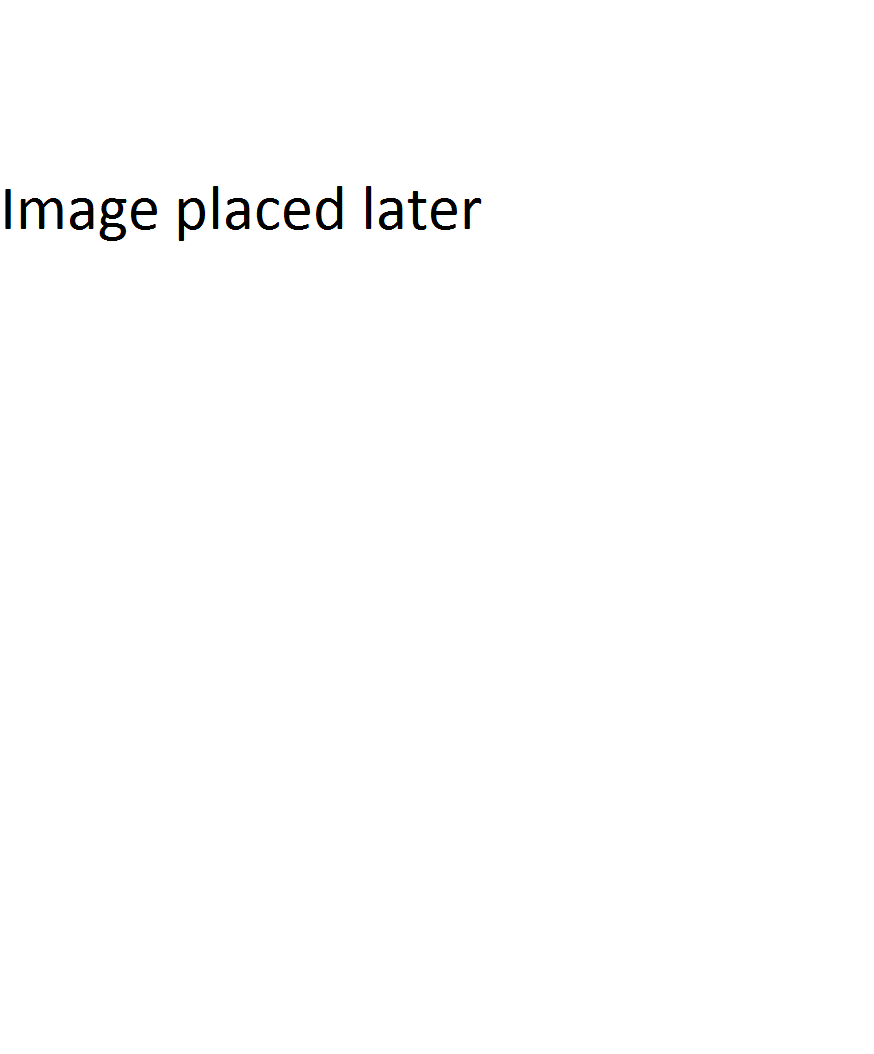
\includegraphics[scale=0.5, width=15cm, keepaspectratio]{./Images/default.png}
		\caption{Domain Model}
		\label{Domain Model}
	\end{figure}

The camera uses a  USB 3.0 connection to connect o the computer.This is due to large amounts of data that needs to be transported quickly.Below shows two pictures of how the eye tribe is connected to the computer.

	\begin{figure}[!ht]
		\centering
		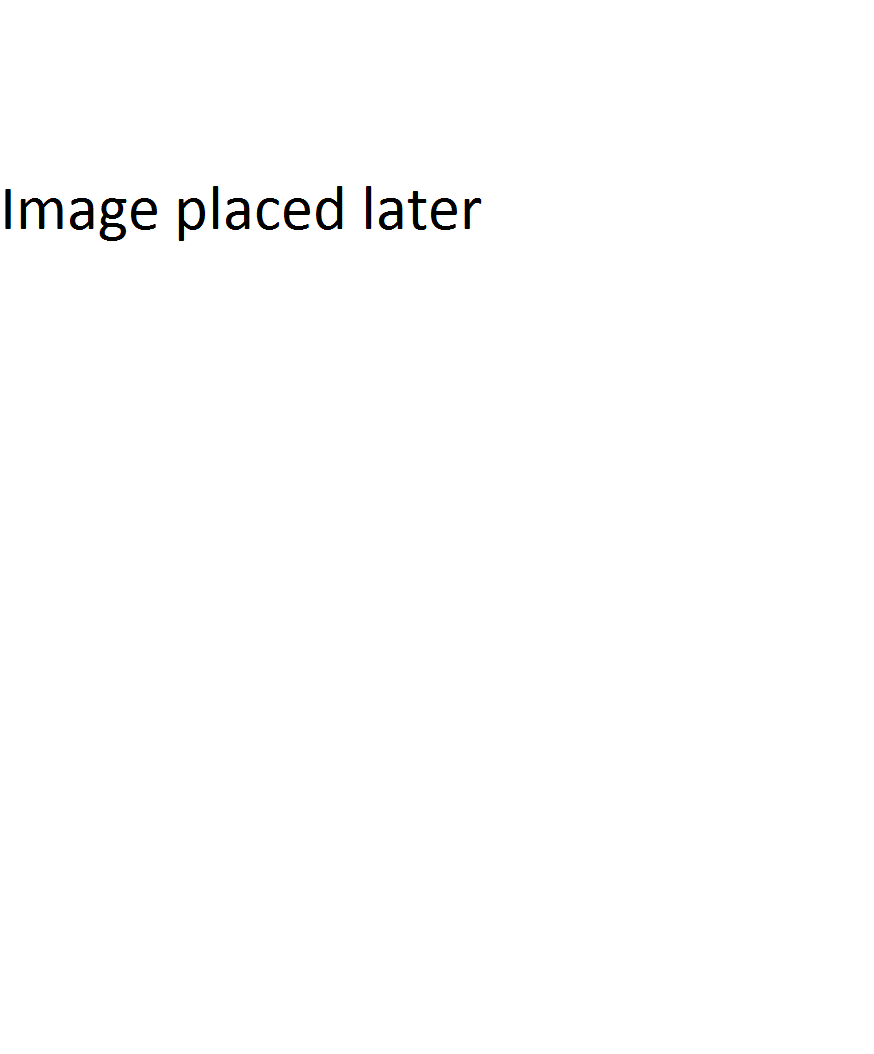
\includegraphics[scale=0.5, width=15cm, keepaspectratio]{./Images/default.png}
		\caption{Domain Model}
		\label{Connection to the computer}
	\end{figure}

	
		\begin{figure}[!ht]
		\centering
		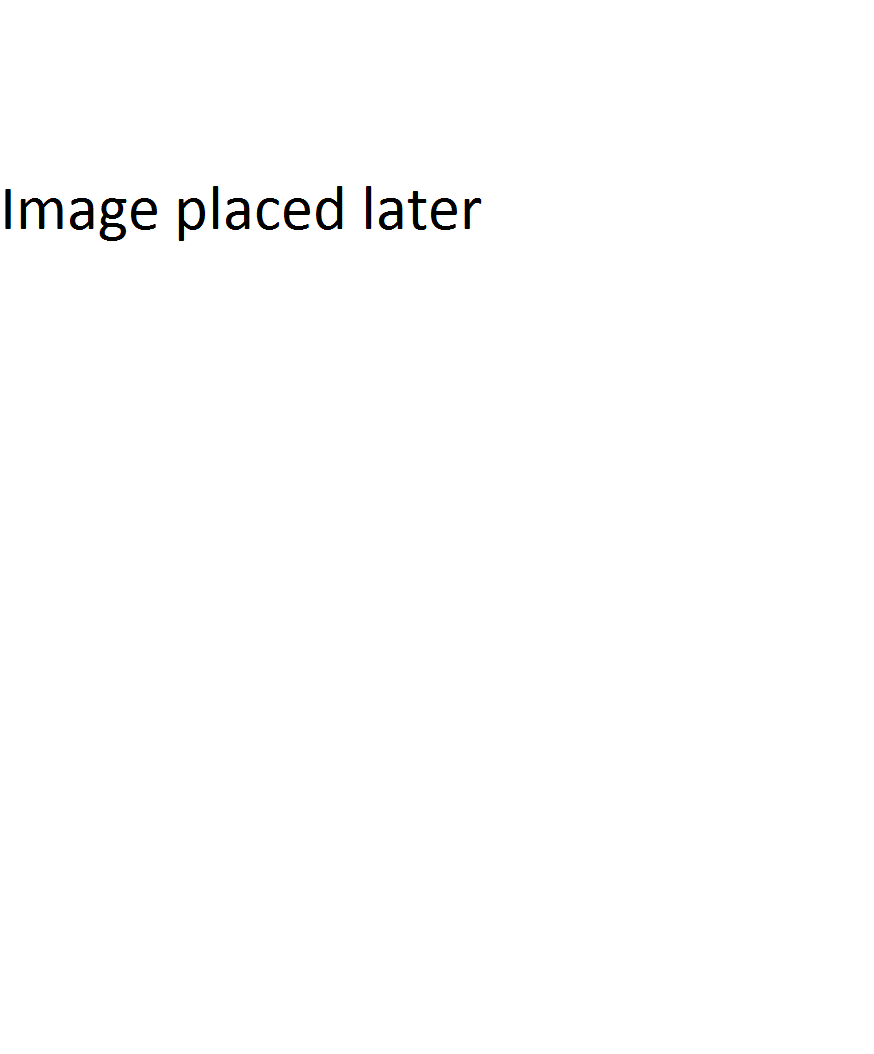
\includegraphics[scale=0.5, width=15cm, keepaspectratio]{./Images/default.png}
		\caption{Domain Model}
		\label{Connection to the Eye tribe camera}
	\end{figure}

		\begin{figure}[!ht]
		\centering
		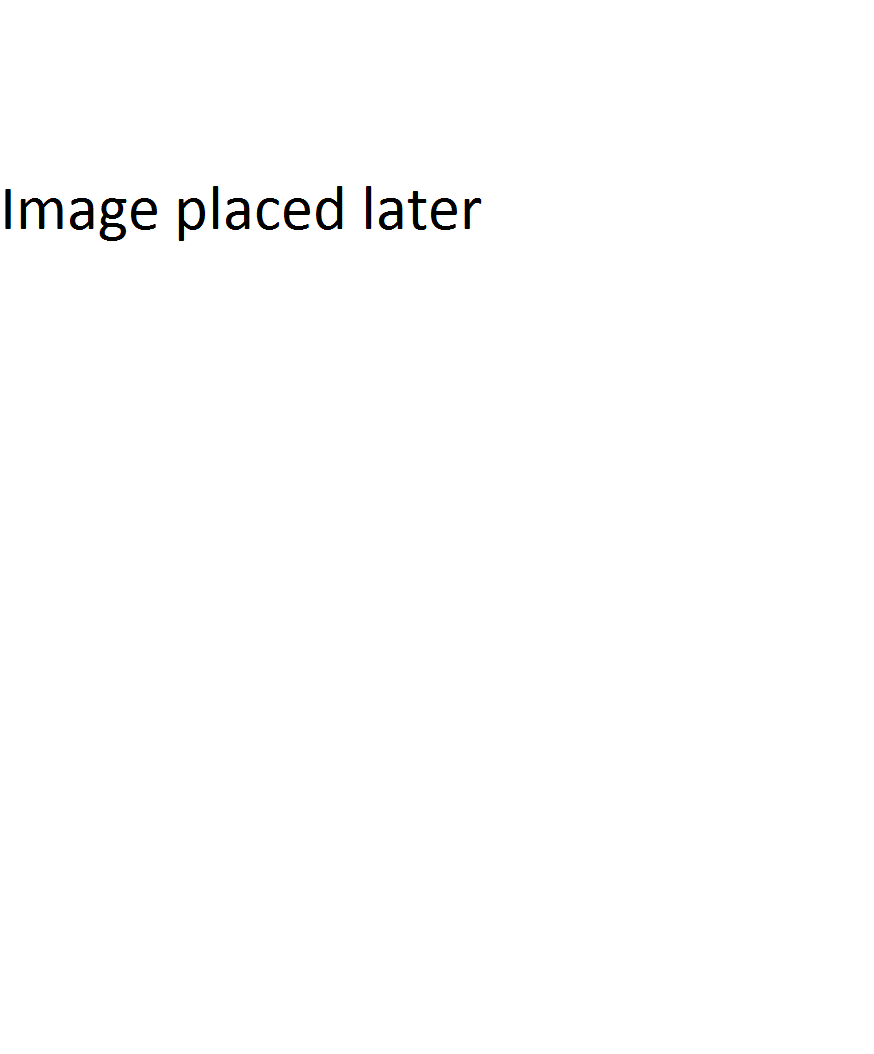
\includegraphics[scale=0.5, width=15cm, keepaspectratio]{./Images/default.png}
		\caption{Domain Model}
		\label{Eyetribe placed on tripod}
	\end{figure}

\subsection{Installation}
Please ensure that you meet the minimum requirements. It is recommended that you meet the recommended requirements as this will ensure that the best performance is achieved.The software can be downloaded from Github.At the moment it is only an executable file but a full installation onto your computer will be developed soon.Follow the steps below to install the eye tracking software on your computer.\\

1)Navigate to \href{https://github.com/MichaelNunes/Neo-Tandem-Tech-Eye-Tracking} and then click on the download as zip button.

	\begin{figure}[!ht]
		\centering
		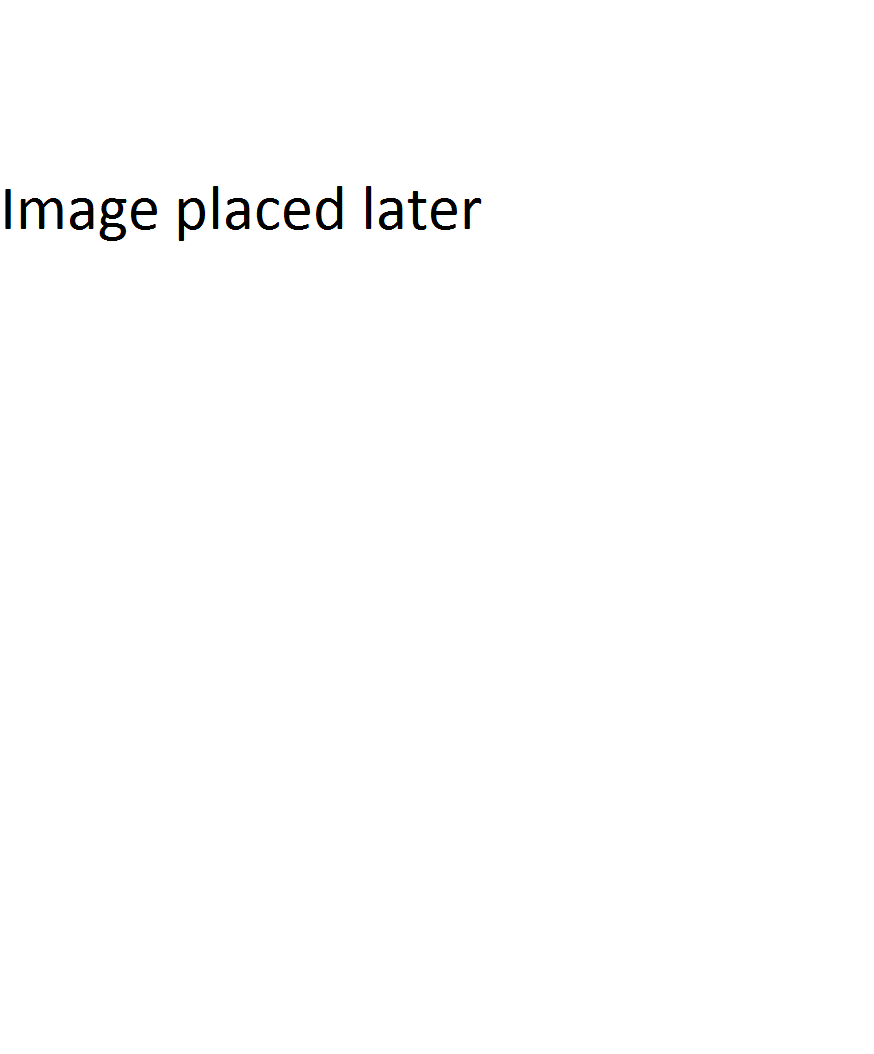
\includegraphics[scale=0.5, width=15cm, keepaspectratio]{./Images/default.png}
		\caption{Domain Model}
		\label{Downloading the files}
	\end{figure}
	
2)Unzip the archive using software of your choice to a folder of your choice

	\begin{figure}[!ht]
		\centering
		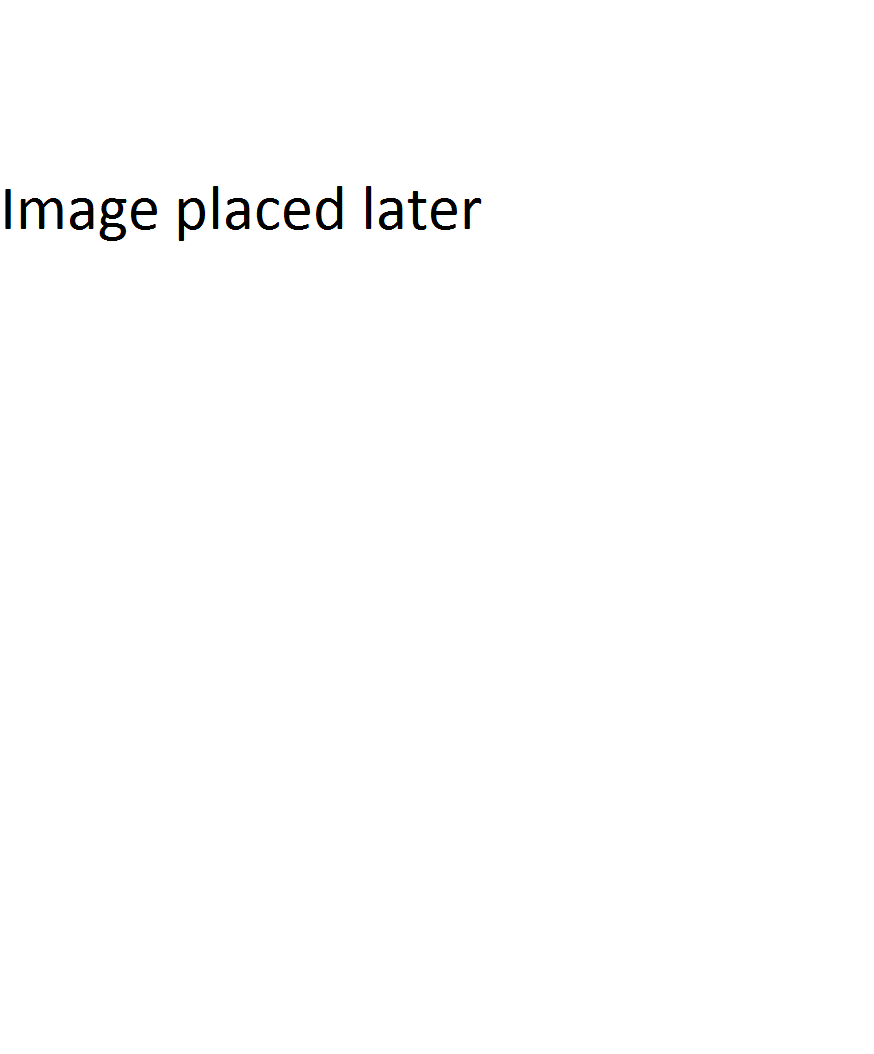
\includegraphics[scale=0.5, width=15cm, keepaspectratio]{./Images/default.png}
		\caption{Domain Model}
		\label{Unzip files}
	\end{figure}

3)Navigate to the following directory: filename/Neo-Tandem-Tech-Eye-Tracking/Final work/Main v2/NTT Eye Tracking/NTT Eye Tracking/bin/Debug.

	\begin{figure}[!ht]
		\centering
		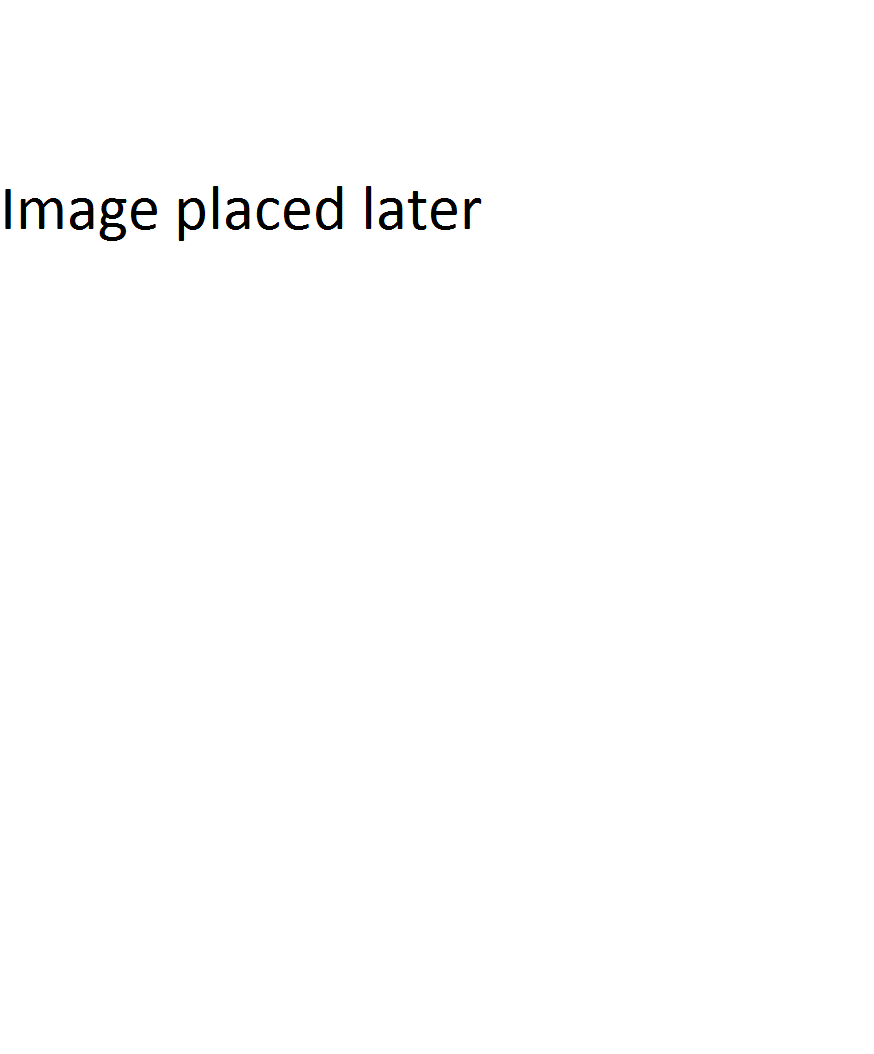
\includegraphics[scale=0.5, width=15cm, keepaspectratio]{./Images/default.png}
		\caption{Navigation to folder}
		\label{Unzip files}
	\end{figure}
	
4)Here you can run the executable called NTT Eye Tracking.exe and the program is run.
	\begin{figure}[!ht]
		\centering
		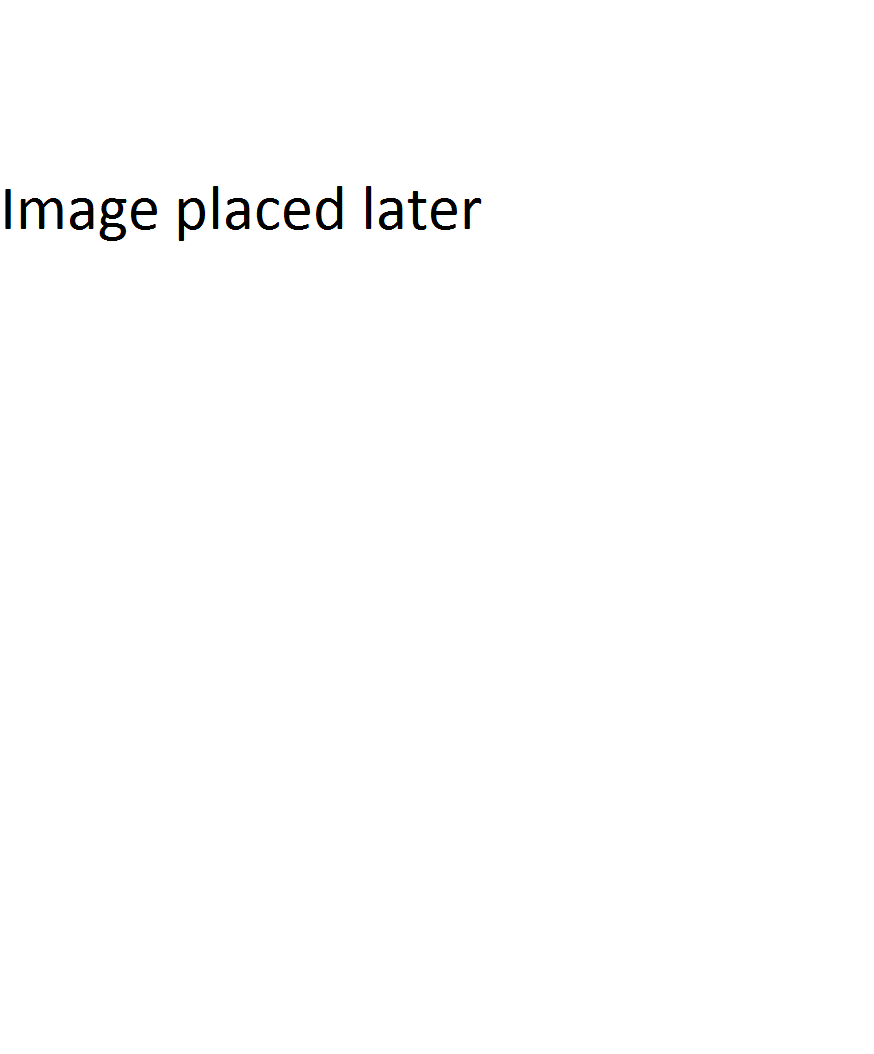
\includegraphics[scale=0.5, width=15cm, keepaspectratio]{./Images/default.png}
		\caption{Running program}
		\label{Unzip files}
	\end{figure}